\section{Fixed-map Pell blocks: a global Gaussian law and its rate}
\label{sec:pell}

Consider the fixed hyperbolic map and associated constants
\[
 T=\begin{pmatrix}3&2\\4&3\end{pmatrix},\qquad
 \alpha=1+\sqrt2,\qquad\lambda=\alpha^2.
\]
For each odd prime $K$, set $N+F\sqrt2=\alpha^K$, so that
$N^2-2F^2=-1$. The modulus $N$ may be composite. Put
$s=F^{-1}\pmod N$, $h=3+2s\pmod N$ and $q=-F\pmod N$.
Then $s^2=2$, and $h$ has exact order $K$ modulo each prime divisor of $N$.
In particular, $h^d-1$ is a unit for $0<d<K$, and $h^d+1$ is a unit for all $d$.

Use Weyl operators
\[
 \begin{gathered}
 (W(a,b)f)(x)=e_N(a(x-b/2))f(x-b),\qquad
 (S_hf)(x)=f(h^{-1}x),\\
 Q_j=\frac1K\sum_{t=0}^{K-1}e^{-2\pi ijt/K}S_h^t.
 \end{gathered}
\]
The explicit symplectic diagonalization in the maintained Pell note takes
the original cosine observable to the odd-sector blocks
\[
 A_j=\left.Q_j\{W(q,1)+W(q,1)^*\}Q_j\right|_{\rm odd},
 \qquad n=\frac{N-1}{2K},\qquad X_j=\sqrt{K/2}\,A_j.
\]
Each sector has dimension $n$, including at composite moduli.
The symmetrized observable preserves parity; an individual Weyl translation
need not do so. All claims here concern these observable blocks.

\begin{theorem}[Global Gaussian limit and rate]
For every fixed integer $r\ge1$, as $K$ tends to infinity through odd primes,
\[
 \sup_{0\le j<K}\left|n^{-1}\operatorname{Tr} X_j^{2r}-(2r-1)!!\right|
 =O_r(K^{-1})+O_r(K^{r+1}/N).
\]
For each fixed odd $m$ and all sufficiently large $K$,
\[
 \sup_j |n^{-1}\operatorname{Tr} X_j^m|
 \le 2^{m/2+1}K^{m/2+1}/(N-1).
\]
Thus the global empirical measures converge weakly to the variance-one
Gaussian, uniformly in the sequential choice of sector.
\end{theorem}

\begin{proof}
The fixed-point Weyl trace identity separates central reciprocal-zero words
from a remainder at most $2^{m/2+1}K^{m/2+1}/(N-1)$. The unit conditions
justify this estimate at composite $N$.

A modular reciprocal relation with $m$ signed terms can be rotated over its
largest cyclic gap. Its polynomial has degree at most $K-K/m$ and coefficient
$\ell^1$ norm at most $m$. If its value at $\lambda$ were nonzero, its algebraic
norm would be a nonzero multiple of $N^2$ but have absolute value at most
$m^2\lambda^{K-K/m}$. Since $N^2\asymp\lambda^K$, this is impossible for
fixed $m$ and large $K$. Hence the relation lifts to characteristic zero.
The minimal polynomial $x^2-6x+1$ takes value $-4$ at $1$, excluding odd
signed relations. The same norm argument shows that a gap exceeding
$2\log_\lambda m$ splits a relation. Bounded-width components then give
$O_r(K^{r-2})$ pinned nonpairable configurations, compared with $K^{r-1}$
paired configurations. Detailed component counting is in the Pell notes.

It remains to control crossing phases without a logarithmic loss.
Let $P_t$ be the Pell sequence, and let $\delta$ be the signed representative
of $d$ modulo $K$. Exactly,
\[
 z_d=e_N(q(h^d-h^{-d}))=e_N(-2P_{2\delta}).
\]
Writing $\delta=(K-1)/2-\ell$ for positive $\delta$ gives
\[
 \frac{P_{2\delta}}{N}
 =\frac{\lambda^{-\ell}}{\sqrt2\alpha}
 \frac{1-\lambda^{-2\delta}}{1-\lambda^{-K}}.
\]
Since $\alpha(1-\lambda^{-1})=2$, summing $|e^{it}-1|\le|t|$ yields
\[
 \sum_{d\bmod K}|z_d-1|
 \le \frac{2\sqrt2\pi}{1-\lambda^{-K}}<9.
\]
Each crossing label difference is uniform under pairing-label averaging,
even when one pair label is pinned. The product inequality for unit phases
therefore gives a mean error at most $9/K$ per crossing, without requiring
independence of different crossings. Repeated-label overcount and
nonpairable words contribute $O_r(K^{-1})$. The stated trace bounds follow.
Gaussian moment determinacy and higher even-moment bounds give weak convergence.
\end{proof}

\begin{theorem}[First fourth-moment correction]
For odd prime $K\ge11$, uniformly in $j$,
\[
 n^{-1}\operatorname{Tr} X_j^4=3-\frac{\gamma}{K}+O(K^3/N),
\]
where
\[
 \gamma=\frac32+2\sum_{\ell\ge0}
 \left[1-\cos\left(\frac{4\pi}{\sqrt2\alpha}\lambda^{-\ell}\right)\right]
 =5.61422069215\ldots.
\]
The following finite formula has an explicit remainder:
\[
 n^{-1}\operatorname{Tr} X_j^4=\frac{N}{N-1}\left(2+S_K-\frac{3}{2K}\right)+R_{4,j},
 \qquad |R_{4,j}|\le \frac{8K^3}{N-1},
\]
\[
 S_K=\frac1K\left(1+2\sum_{\delta=1}^{(K-1)/2}
                         \cos(4\pi P_{2\delta}/N)\right).
\]
\end{theorem}

\begin{proof}
Four-term reciprocal modular relations lift for $K\ge11$, since
$\lambda^{K/4}(1-\lambda^{-K})^2>64$. A lifted four-term relation pairs
because $\lambda>3$. Two pairings are noncrossing and one is crossing.
The six balanced all-equal sign words are counted twice; subtracting that
overcount gives $3/(2K)$. The noncentral fixed-point trace estimate gives
$R_{4,j}$. Reindexing the exact Pell ratio yields the cosine series.
The summed finite-argument error is $O(N^{-1})$ before division by $K$,
and the omitted cosine tail is $O(\lambda^{-K})$. With
$a=4\pi/(\sqrt2\alpha)$, the nonnegative tail after $J$ terms is at most
$a^2\lambda^{-2J}/(1-\lambda^{-2})$.
\end{proof}

\paragraph{Verification and scope.}
The independent orbit-matrix verifier includes nontrivial sectors and
$N=8119=23\cdot353$. Its matrix-power and eigenvalue moments are numerical
checks, not replacements for the proofs. The displayed decimal for $\gamma$ is now independently enclosed by
pure-integer interval arithmetic: Machin arctangent bounds, integer square
root, outward arithmetic, cosine Taylor remainders, and a geometric tail.
The separate matrix diagnostics still use floating-point arithmetic. Existing Lean certificates concern explicit finite word traces;
they do not formalize these general limit theorems. Priority remains unverified.
Neither this Gaussian global density nor an exact all-order trace formula
establishes local spacings or Heisenberg-scale universality for the propagator.

\IfFileExists{../assets/figures/pell_fourth_moment.png}{%
\begin{figure}[ht]
\centering
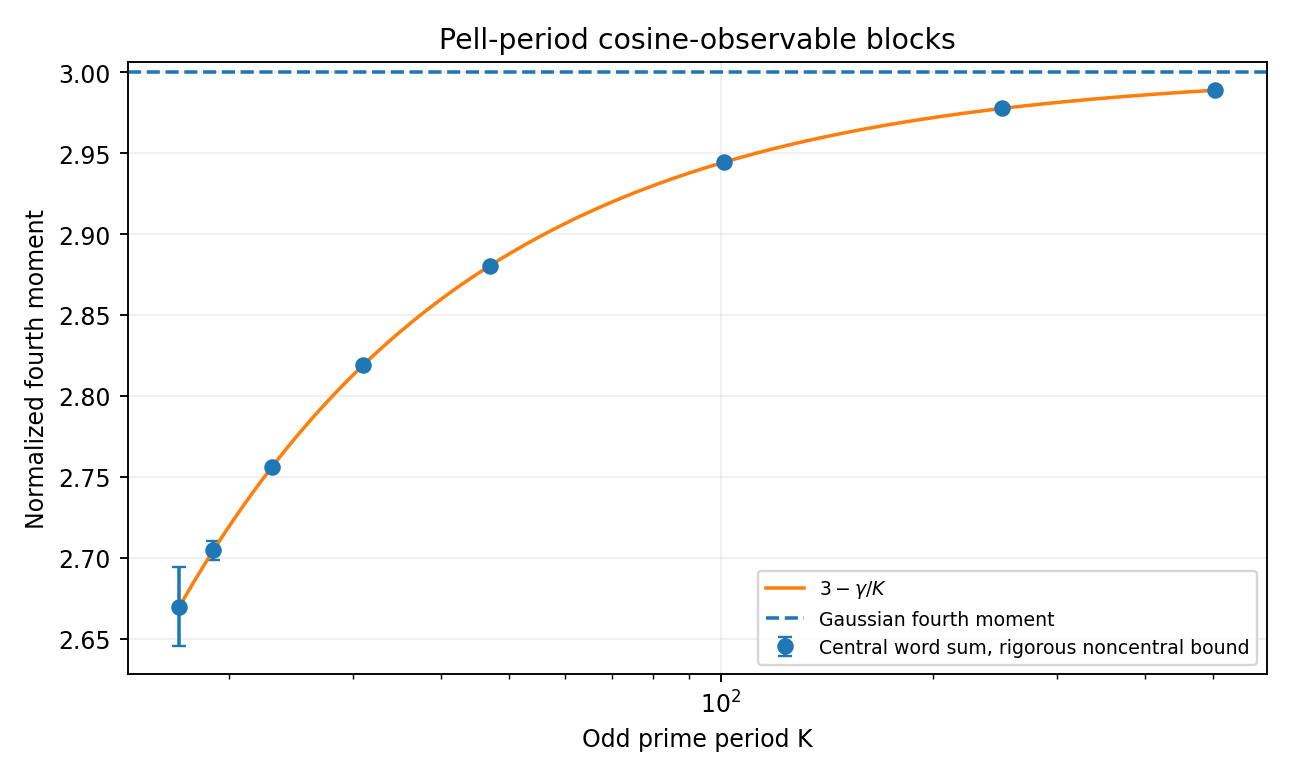
\includegraphics[width=.87\linewidth]{../assets/figures/pell_fourth_moment.png}
\caption{Central fourth-moment word sums with the explicit noncentral bound,
compared with $3-\gamma/K$. This is not a level-spacing plot.}
\end{figure}}{}
